\documentclass{amsart}
\title{Security of cyclotomic extensions against the [ELOS]
attack on RLWE}
\author{Hao Chen \and  Kristin Lauter \and Kate Stange}

\usepackage{macros}
\usepackage{float}
\usepackage{url}
\usepackage{placeins}

\begin{document}
\maketitle

\section{Introduction}

We expect that under some mild assumptions, the image of a discrete Gaussian error distribution under the ring maps $\cO_K \to \bF_q$ for a split prime $q$ will be non-distinguishable from the uniform distribution $U(\bF_q)$.

To aid the analysis, we use another class of distribution instead of discrete Gaussian distributions over the integers.

Tools: Fourier analysis on finite fields.

\iffalse
\section{Review: Fourier analysis for 2-power
cyclotomics}

Let $n$ be an integer and let $q$ be a prime with $q \equiv 1 \pmod{n}$, and let $\alpha$ be any primitive $n$-th root of unity in $\bF_q$. In this section we are going to explore the distribution of
\[
    e(\alpha) = e_0 + e_1 \alpha + \cdots + e_{n-1} \alpha^{n-1},
\]
where the $e_i$ are sampled from a discrete Gaussian $D_{\bZ,s}$ modulo $q$. For simplicity,
we are going to assume that for every index $i$, $e_i$ takes on value 0 with probability 1/2, and $e_i = \pm 1$ with probability 1/4 each. Let $P(t) = Prob(e(\alpha) = t)$, then $P(t): \bF_q \to \bR$ is a function, so we could take its Fourier transform.

\begin{Lemma}
\[
    \hat{P}(s) = \prod_{i=0}^{n-1} \cos^2 \left(\frac{\alpha^i \pi s}{q} \right)
\]
\end{Lemma}

We  consider a more general question: let ${\bf a} = (a_1,\cdots a_n)$ be a vector of integers whose residues modulo $q$ are distinct, ($q = poly(n)$).

\begin{align*}
   p_{a} : \bF_q & \to \bR \\
   s & \mapsto \prod_{i=1}^n \cos^2 \left(\frac{a_i \pi s}{q} \right).
\end{align*}

By ``bound'', I mean $\hat{P}$ should be $l_1$ or $l_2$ close to the delta-function.

Note that the assumption that $a_i$ are distinct can not be dropped, otherwise, for example, the l-2 norm squared will be approximated by
\[
    const \cdot q \cdot \int_{0}^{2 \pi} \cos^{4n}(x) dx,
\]
and the last term is asymptotically $\frac{c}{\sqrt{n}}$. So when $q = \Omega(n)$ the product will approch infinity as $n \to \infty$. \\ \\

Note that by the evenness of $\cos$ we may assume $a_i \in [0, q/2)$.

Another note: also we don't want the $a_i$'s to be too small, like $1,2, \cdots, n$. So we will make the assumption (reasonable) that at least one $a_i$ has its reduced representative to be at least $q/n$ (say).

By rotation if necessary, we may assume that
$$1 =\alpha_0 < \alpha_1 \cdots < \alpha_{n-1}.$$
\fi

\section{After introduction}

Suppose $f$ is a real-valued function on $\bF_q$. The Fourier transform of $f$ is defined as
\[
    \hat{f}(s) = \sum_{a \in \bF_q} f(a) \bar{\chi_s}(a),
\]
where $$\chi_s(a) := e^{2 \pi i as/q}$$

We have the inversion formula:
\[
    f(a) = \frac{1}{q} \sum_{s \in \bF_q} \hat{f}(s)\chi_s(a).
\]

Let ${\bf 1}$ denote the constant function $f \equiv 1$, and let $\delta$ denote the characteristic function of the
one-point set $\{0\} \subseteq \bF_q$. We recall some basic properties of the Fourier transform:

\begin{Prop} \hfill \\
\begin{enumerate}
\item The transform of the $\delta$ function is $\hat{\delta} = {\bf 1}$.

\item The transform of {\bf 1} is $\hat{{\bf 1}} = q\delta$; if $U$ the uniform distribution over $\bF_q$, then $\hat{U} = \delta$.

\item convolution becomes product.

%\item Plancherel's formula states that
%$||f||_2 = \frac{1}{q} ||\hat{f}||_2$.

%\item $\hat{f(a - \lambda)}(s) =  \bar{\chi_s(\lambda)} f(s)$.
\end{enumerate}
\end{Prop}

Next we introduce a class of distributions indexed by even integers $k \geq 2$, aiming at approximating discrete Gaussians over the integers. Here $k$ plays the role of
the standard deviation $\sigma$ for discrete Gaussians.

\begin{Definition}
For any even integer $k \geq 2$, $\cV_k$ is the distribution over $\bZ$ such that

$$\prob(\cV_k = m) =  \begin{cases} {k}\choose{m+\frac{k}{2}} &\mbox{if } |m| \leq \frac{k}{2} \\
0 & \mbox{otherwise}  \end{cases}$$

\end{Definition}
When $q$ is a prime such that $q > k$, we abuse notations and let $\cV_k: \bF_q \to \bR$ denote the probability density function of the distribution $`\cV_k'$ over $\bF_q$ defined by the same formula.

\begin{figure}[h!]
\centering
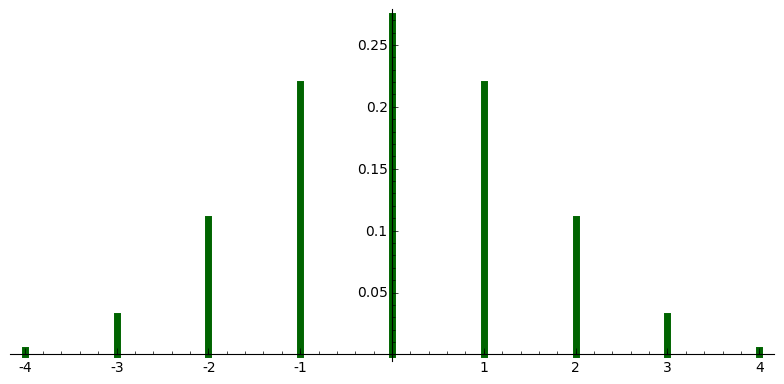
\includegraphics[width = 0.5\textwidth]{v8.png}
\caption{Probability density function of $\cV_8$}
\end{figure}


\begin{Lemma}
For all even integers $k \geq 2$,
$$\hat{\cV_k}(s)  = \cos \left(\frac{\pi s}{q}\right)^k, (\forall s \in \bF_q).$$
\end{Lemma}

\begin{proof}
Routine calculation.
\end{proof}

Now we consider the error distribution we obtained from mapping RLWE errors to $\bF_q$.

\begin{Definition}
Suppose ${\bf a} = a_1, \cdots ,a_n$ is a vector in $\bF_q^n$. Define the following random variable with
values in $\bF_q$
\[
    e({\bf a}, k, q) := \sum_{i=1}^n a_i e_i \pmod {q}
\]
where the $e_i$ are independent variables with distribution $\cV_k$. Let $E$ denote its probability density function:
$E(b) = \prob(e = b)$ for $b \in \bF_q$.
\end{Definition}

Next, using the fact that the probability of a sum of two varaibles is a convolution, we prove
\begin{Lemma}
\[
    \hat{E_{{\bf a}, k, q}}(s) = \prod_{i=1}^{n} \cos \left(\frac{ a_i \pi s}{q} \right)^k
\]
In particular, $\hat{E}(0) = 1$ for all ${\bf a}$, $k$ and $q$.
\end{Lemma}

\begin{proof}
Routine calculation.
\end{proof}





%\begin{equation*}
%\label{eq:1}
%    ||P - U||_2  = \frac{1}{q}||\hat{P} - \delta||_2.
%\end{equation*}

Next we restrict our attention to cyclotomic fields. Let
$m \geq 1$ be an integer and let $q \equiv 1 \pmod{m}$ be a prime. Then $q$ splits completely in the cyclotomic field $K = \bQ(\zeta_m)$. Let $\alpha \in \bF_q$ be a primitive $n$-th root of unity. In the following discussion, we will take $k =2$, and will take
\[
    e = e(\alpha) = \sum_{i=0}^{n-1} e_i \alpha^i.
\]
Let $E$ denote the density function of $e$. Recall that $U$ denotes the density function of the uniform distribution: $U(a) = 1/q$ for all $a \in \bF_q$.Now We can compute $(E - U)(a)$ for any $a \in \bF_q$ using the Fourier inversion formula, using the notations in the beginning of this section,

\begin{align*}
    E(a) - U(a) &= \frac{1}{q} \sum_{s \in \bF_q} (\hat{E}(s) - \hat{U}(s) )\chi_s(a) \\
& = \frac{1}{q} \sum_{s \in \bF_q} (\hat{E}(s) - \delta(s) )\chi_s(a) \\
& = \frac{1}{q} \sum_{s \in \bF_q, s \neq 0} \hat{E}(s) \chi_s(a)
\end{align*}

Since $|\chi_s(a)| \leq 1$ for all $a, s$, we have (very importantly)
\[
    \boxed{|E(a) -  1/q| \leq \frac{1}{q}  \sum_{s \in \bF_q, s \neq 0}  |\hat{E}(s)| =: \epsilon(m,q,\alpha), \, (\forall a \in \bF_q)}
\]
The punchline is: $\epsilon(m,q,\alpha)$ is usually negligably small, and when it is, the distribution $e$ is computationally indistinguishable from the uniform distribution over $\bF_q$. The following is a table of data, to demonstrate how small it is.

\FloatBarrier
\begin{table}[H]
\begin{tabular}{c|c|c}
$m$ & $q$ & $[\log_2(\epsilon(m,q, \alpha))]$ \\
\hline
244 & 1709 & $-230$ \\
101 & 1213 & $-177$ \\
256 & 3329 & $-194$ \\
256 & 14081 & $-208$ \\
55 & 10891  & $-44$ \\
197 & 3547 & $-337$ \\
96 & 4513 & $-35$ \\
160 & 20641 & -61 \\
145 & 19163 & $-176$ \\
101 & 101 & $-4$ \\
13 & 1000039 & $-12$
\end{tabular}
\end{table}

On row $-1$ and $-2$ from the above table, we can see the effect of taking the ramified prime, or taking $q >> n$.



\begin{remark}
It is possible to generalize this cryptoanalysis to higher degree primes, where we are looking at general finite fields $\bF_{q^r}$. In this situation we should interpret
$\chi_s(a) = e^{2 \pi i Tr(as)/q}$. Separability tells us this is an isomorphism between $\bF_q$ and its dual, and we can define the Fourier transform this way. So everything goes through? We just want to add a trace to everything, i.e.,

\[
    \hat{E_{{\bf a}, k, q}}(s) = \prod_{i=1}^{n} \cos \left(\frac{ \pi Tr(a_i s) }{q} \right)^k
\]
Note this is well-defined when $k$ is even, which we always assume.
\end{remark}


We have a table for degree 2 primes.
\FloatBarrier
\begin{table}[H]
\begin{tabular}{c|c|c}
$m$ & $q$ & $[\log_2(\epsilon(m,q, \alpha))]$ \\
\hline
53 & 211 & -61 \\
55 & 109 & -48 \\
63 & 881 & -33 \\
64 & 127 & -37 \\
64 & 191 & -35 \\
64 & 383 & -31 \\
256 & 127 & -193 \\
256 & 383 & -180 \\
256 & 641 & -136 
\end{tabular}
\end{table}



\newpage

\section{References}

\url{https://en.wikipedia.org/wiki/Fourier_transform_on_finite_groups}

\url{http://arxiv.org/pdf/0909.5471v1.pdf}

\url{https://books.google.com/books?id=-B2TA669dJMC&pg=PA251#v=onepage&q&f=false}

\end{document}
